% !TEX root = ./Vorlesungsmitschrift AGLA 2.tex  
\lecture{Fr 19.06. 10:15}{}
\file{Dualität}
\section{Dualität}
Sei \( K \) ein Körper und \( L\subseteq \projectionspaceover{2}{K} \) eine projektive Gerade. Seien \( (x_0,x_1,x_2) \) homogene Koordinaten in \( \projectionspaceover{2}{K} \) und \( L=\projectionspace{U} \) mit \( U\subseteq K^3 \) ein \( 2 \)-dimensionaler Untervektorraum. Dann gibt es \( (a_0,a_1,a_2)\in K^3 \), sodass \( U\untervektorraum K^3 \) gegeben ist durch
\begin{equation*}
  a_0x_0 +a_1x_1+a_2x_2=0
\end{equation*}
und
\begin{equation*}
  L=\Set{(x_0:x_1:x_2)\in \projectionspaceover{2}{K}|a_0x_0+a_1x_1+a_2x_2=0}.
\end{equation*}
Ist \( \lambda\in \fieldwithoutzero{K} \), so definiert das Tupel \( (\lambda a_0,\lambda a_1,\lambda a_2) \) ebenfalls die Gerade
\begin{equation*}
  L=\Set{(x_0,x_1,x_2)\in \projectionspaceover{2}{K}|\lambda a_0 x_0+\lambda a_1 x_1+\lambda a_2 x_2=0}.
\end{equation*}
Wir verstehen \( (a_0:a_1:a_2) \) als Element in \( \projectionspaceover{2}{K} \) und erhalten eine Bijektion
\begin{equation*}
  \begin{split}
    \Set{\text{projektive Geraden \( L\subseteq \projectionspaceover{2}{K} \)}}&\leftrightarrow \Set{\text{Punkte in \( \projectionspaceover{2}{K} \)}}\\
    L=\Set{(x_0,x_1,x_2)\subseteq \projectionspaceover{2}{K}|a_0x_0+a_1x_1+a_2x_2=0}&\leftrightarrow (a_0:a_1:a_2)\in \projectionspaceover{2}{K}.
  \end{split}
\end{equation*}
Ist \( p=(x_0,x_1,x_2)\in \projectionspaceover{2}{K} \) eine Punkt, so können wir die projektive Gerade
\begin{equation*}
  \Set{(a_0:a_1:a_2)\in \projectionspaceover{2}{K}|a_0x_0+a_1x_1+a_2x_2=0}
\end{equation*}
zuordnen. Wir erhalten eine Bijektion
\begin{align*}
  \varphi\maps \Set{\text{projektive Unterräume von \( \projectionspaceover{2}{K} \)}}&\to\Set{\text{projektive Unterräume von \( \projectionspaceover{2}{K} \)}}\\
  \emptyset&\mapsto \projectionspaceover{2}{K}\\
  \projectionspaceover{2}{K}&\mapsto \emptyset\\
  L=\Set{(x_0:x_1:x_2)|a_0x_0+a_1x_1+a_2x_2=0}&\mapsto (a_0:a_1:a_2)\\
  \projectionspaceover{2}{K}\ni (x_0:x_1:x_2)\mapsto \Set{(a_0:a_1:a_2)\in \projectionspaceover{2}{K}|a_0x_0+a_1x_1+a_2x_2=0}.
\end{align*}
Ist \( p\in \projectionspaceover{2}{K} \) und \( L\subset \projectionspaceover{2}{K} \) eine projektive Gerade, so gilt
\begin{equation*}
  p\in L\iff \varphi(L)\in \varphi(p)
\end{equation*}
\begin{figure}[H]
  \centering
  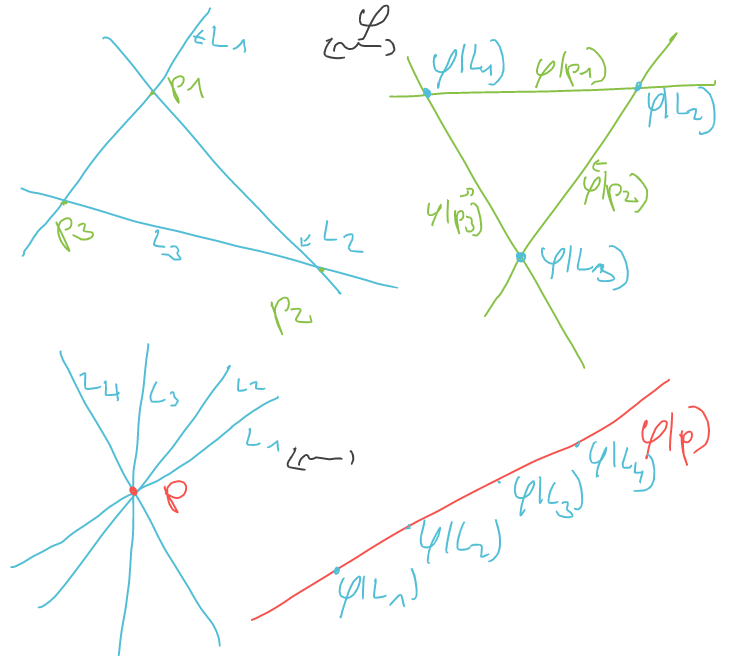
\includegraphics[width=0.9\linewidth]{dualitaet_enthaltungssatz}
  \label{fig:dualitaet_enthaltungssatz}
\end{figure}
\subsection*{Dualisierung des Satzes von Desargues.}
\begin{erinnerung*}[Satz von Desargues]
  Seien \( p_1,p_2,p_3,p_1',p_2',p_3'\in \projectionspaceover{2}{K} \) paarweise verschiedene Punkte, sodass die Geraden \( p_1\vee p_1' \), \( p_2\vee p_2' \), \( p_3\vee p_3' \) sich paarweise in einem Punkt \( z \) schneiden. Dann liegen die Schnittpunkte
  \begin{align*}
    a&\definedas (p_1\vee p_2)\cap (p_1'\vee p_2')\\
    b&\definedas (p_2\vee p_3)\cap (p_2'\vee p_3')\\
    c&\definedas (p_3\vee p_1)\cap (p_3'\vee p_1')
  \end{align*}
  auf einer gemeinsamen Geraden \( L \). 
\end{erinnerung*}
Wir \enquote{dualisieren} den Satz von Desargues. Sei \( \varphi \) wie oben definiert. Setze
\begin{align*}
  Z_i&=\varphi(p_i)\quad 1\leq i\leq 3\\
  Z_i'&=\varphi(p_i')\quad 1\leq i\leq 3.
\end{align*}
Dann sind \( Z_1,Z_2,Z_3,Z_1',Z_2',Z_3' \) paarweise verschiedene Geraden mit
\begin{align*}
  Z_1\cap Z_1'&=\varphi(p_1\vee p_1')\\
  Z_2\cap Z_2'&=\varphi(p_2\vee p_2')\\
  Z_3\cap Z_3'&=\varphi(p_3\vee P_3').
\end{align*}
Die Punkte \( Z_1\cap Z_1' \), \( Z_2\cap Z_2' \), \( Z_3\cap Z_3' \) sind enthalten in der Geraden \( \varphi(Z) \), mit
\begin{equation*}
  z=(p_1\vee p_1')\cap (p_2\vee p_2')\cap (p_3\vee p_3').
\end{equation*}
Weiter gilt
\begin{align*}
  \phi((p_1\vee p_2)\cap (p_1'\vee p_2'))&=\varphi(p_1\vee p_2)\vee \varphi(p_1'\vee p_2')\\
  &=(Z_1\cap Z_2)\vee (Z_1'\cap Z_2')\\
  \varphi(b)&=(Z_2\cap Z_3)\vee (Z_2'\cap Z_3')\\
  \varphi(c)&=(Z_3\cap Z_1)\vee (Z_3'\cap Z_1').
\end{align*}
Nach dem Satz von Desargues liegen \( a,b,c \) auf einer Geraden, \dh \( \varphi(a) \), \( \varphi(b) \) und \( \varphi(c) \) schneiden sich in einem Punkt.

Seien \( Z_1,Z_2,Z_3,Z_1',Z_2',Z_3' \) paarweise verschiedene Geraden, sodass die Schnittpunkte \( Z_1\cap Z_1' \), \( Z_2\cap Z_2' \), \( Z_3\cap Z_3' \) paarweise verschieden sind und auf einer Geraden liegen. Dann gibt es paarweise verschiedene Punkt \( p_1,p_2,p_3,p_1',p_2',p_3'\in \projectionspaceover{2}{K} \), die die Annahmen des Satzes von Desargues erfüllen. WÄhle dazu
\begin{align*}
  p_i\definedas \inverse{\varphi}(Z_i)\quad 1\leq i\leq 3\\
  p_i'\definedas \inverse{\varphi}(Z_i')\quad 1\leq i\leq 3.
\end{align*}
\begin{satz}[Dualer Satz von Desargues]
  Seien \( Z_1,Z_2,Z_3,Z_1',Z_2',Z_3' \) paarweise verschiedene Geraden, sodass die Schnittpunkte \( Z_1\cap Z_1' \), \( Z_2\cap Z_2' \), \( Z_3\cap Z_3' \) paarweise verschieden sind und auf einer Geraden liegen. Dann gehen die Geraden \( (Z_1\cap Z_2)\vee (Z_1'\cap Z_2') \), \( (Z_2\cap Z_3)\vee (Z_2'\cap Z_3') \), \( (Z_3\cap Z_1)\vee (Z_3'\cap Z_1') \) durch einen gemeinsamen Punkt.
\end{satz}
\begin{bemerkung*}
  Nach Dualisierung erhalten wir also die Umkehrung zum Satz von Desargues.
\end{bemerkung*}
\begin{satz}[Brianchon]
  (dual zum Satz von Pappos) Seien \( p,p'\in \projectionspaceover{2}{K} \) unterschiedliche Punkte und \( Z_1,Z_2,Z_3,Z_1',Z_2',Z_3'\subseteq \projectionspaceover{2}{K} \) paarweise verschiedene Geraden 
  \begin{align*}
    p&=Z_1\cap Z_2\cap Z_3\\
    p'&=Z_1'\cap Z_2'\cap Z_3'.
  \end{align*}
  Dann gehen die Geraden \( (Z_1\cap Z_2')\vee (Z_1'\cap Z_2) \), \( (Z_2\cap Z_3')\vee (Z_2'\cap Z_3) \) und \( (Z_3\cap Z_1')\vee (Z_3'\cap Z_1)\) durch einen gemeinsamen Punkt.
  
\end{satz}
\begin{proof}
  Die Punkte \( \varphi(Z_1),\varphi(Z_2),\varphi(Z_3),\varphi(Z_1'),\varphi(Z_2'),\varphi(Z_3') \) sind paarweise verschieden und es gilt
  \begin{align*}
    \varphi(Z_1),\varphi(Z_2),\varphi(Z_3)&\in \varphi(p)\\
    \varphi(Z_1'),\varphi(Z_2'),\varphi(Z_3')&\in \varphi(p').
  \end{align*}
  Nach dem Satz von Pappos sind die Punkte
  \begin{align*}
    a&\definedas(\varphi(Z_1)\vee \varphi(Z_2'))\cap (\varphi(Z_1')\vee \varphi(Z_2))\\
    b&\definedas (\varphi(Z_2)\vee \varphi(Z_3'))\cap (\varphi(Z_2')\vee \varphi(Z_3))\\
    c&\definedas (\varphi(Z_3)\vee \varphi(Z_1'))\cap (\varphi(Z_3')\vee \varphi(Z_1))
  \end{align*}
  in einer Geraden \( L \) enthalten. Es ist
  \begin{align*}
    a&=\varphi(Z_1\cap Z_2')\cap \varphi(Z_1'\cap Z_2)\\
    &=\varphi((Z_1\cap Z_2')\vee (Z_1'\cap Z_2)).
  \end{align*}
  Also gehen die Geraden \( (Z_1\cap Z_2')\vee (Z_1'\cap Z_2) \), \( (Z_2\cap Z_3')\vee (Z_2'\cap Z_3) \) und \( (Z_3\cap Z_1')\vee (Z_3'\cap Z_1)\) durch einen gemeinsamen Punkt.
  
\end{proof}
\file{Korrelationen}
Die an Anfang dieses Abschnitts konstruierte Bijektion
\begin{equation*}
  \varphi\maps \Set{\text{projektive Unterräume von \( \projectionspaceover{2}{K} \)}}\to\Set{\text{projektive Unterräume von \( \projectionspaceover{2}{K} \)}}
\end{equation*}
ist eine Beispiel für eine Korrelation.
\begin{definition*}
  Sei \( \projectionspace{V} \) ein projektiver Raum mit \( V \) ein \( K \)-Vektorraum. Schreibe \( \projectionspaces{V} \) für die Menge von projektiven Unterräumen von \( V \). Wir nennen eine bijektive Abbildung
  \begin{equation*}
    \sigma\maps \projectionspaces{V}\to \projectionspaces{V}
  \end{equation*}
  eine Korrelation in \( \projectionspace{V} \), falls es für alle \( Z,Z'\in \projectionspaces{V} \) gilt
  \begin{equation*}
    Z'\subseteq Z\iff \sigma(Z')\supseteq \sigma(Z).
  \end{equation*}
\end{definition*}
\begin{bemerkung*}
  Ist \( \varphi\maps \projectionspaces{V}\to \projectionspaces{V} \) eine Korrelation, dann auch \( \inverse{\sigma} \).
\end{bemerkung*}
\begin{lemma}
  Sei \( \projectionspace{V} \) ein projektiver Raum, \( \sigma\maps \projectionspaces{V}\to \projectionspaces{V} \) eine Korrelation und \( Z,Z'\in \projectionspaces{V} \) projektive Unterräume. Dann gilt
  \begin{enumerate}
    \item \label{dimension_unter_korrelation} \( \projectivedim-{\sigma(Z)}=\projectivedim-{\projectionspace{V}}-(\projectivedim-{Z}+1) \)
    \item \label{schnitt_unter_korrelation} \( \sigma(Z\cap Z')=\sigma(Z)\vee \sigma(Z') \)
    \item \label{verbindung_unter_korrelation} \( \sigma(Z\vee Z')=\sigma(Z)\cap \sigma(Z') \).
  \end{enumerate}
\end{lemma}
\begin{proof}
  \begin{proofdescription}
    \item[\ref{dimension_unter_korrelation}] Sei \( n\definedas \projectivedim-{\projectionspace{V}} \), \( k\definedas \projectivedim-{Z} \). Wähle projektive Unterräume \( Z_i \), \( -1\leq i\leq n \) mit \( Z_{-1}=\emptyset \), \( Z_k=Z \), \( Z_n=\projectionspace{V} \) und \( \projectivedim-{Z_i}=i \), \( -1\leq i\leq n \) und 
    \begin{equation*}
      \emptyset =Z_{-1}\subseteq Z_0\subseteq Z_1\subseteq \dotsb\subseteq \equalto{Z}{Z_k}\subseteq Z_{k+1}\subseteq\dotsb\subseteq Z_n=\projectionspace{V}.
    \end{equation*}
    Dann ist \( Z_i\neq Z_{i+1} \) für \( 1\leq i\leq n-1 \) und
    \begin{equation*}
      \sigma(Z_{-1})\supseteq \sigma(Z_0)\supseteq \sigma(Z_1)\supseteq \dotsb\supseteq \sigma(Z_k)\supseteq\dotsb\supseteq \sigma(Z_n).
    \end{equation*}
    Da \( \sigma \) Bijektion ist, gilt \( \sigma(Z_i)\neq \sigma(Z_{i+1}) \), \( -1\leq i\leq n \), also \( \projectivedim-{\sigma(Z_i)}\geq \projectivedim-{\sigma(Z_{i+1})}+1 \). Daraus folgt
    \begin{equation*}
      \projectivedim-{\sigma(Z)}=\projectivedim{\projectionspace{V}}-(\projectivedim-{Z}+1).
    \end{equation*}
    \item[\ref{schnitt_unter_korrelation}] Seien \( Z,Z'\in \projectionspaces{V} \). Es ist \( Z\cap Z'\subseteq Z,Z' \), also
    \begin{equation*}
      \sigma(Z\cap Z')\supseteq \sigma(Z),\sigma(Z').
    \end{equation*} \( 
      \sigma(Z\cap Z') \) ist projektiver Raum, also 
      \begin{equation*}
        \sigma(Z\cap Z')\supseteq \sigma(Z)\vee \sigma(Z').
      \end{equation*}
      Aus
      \begin{equation*}
        \sigma(Z),\sigma(Z')\subseteq \sigma(Z)\vee \sigma(Z')
      \end{equation*}
      folgt nach Anwendung von \( \inverse{\sigma} \)
      \begin{equation*}
        Z\cap Z'\supseteq \inverse{\sigma}(\sigma(Z)\vee \sigma(Z'))
      \end{equation*}
      und damit
      \begin{equation*}
        \sigma(Z\cap Z')\subseteq \sigma(Z)\vee \sigma(Z').
      \end{equation*}
      \item[\ref{verbindung_unter_korrelation}] Es ist \( Z,Z'\subseteq \sigma(Z)\cap \sigma(Z') \), also \( \sigma(Z\vee Z')\subseteq \sigma(Z)\cap \sigma(Z') \). Wende nun \( \inverse{\sigma} \) an auf
      \begin{equation*}
        \sigma(Z)\cap \sigma(Z')\subseteq \sigma(Z),\sigma(Z')
      \end{equation*}
      und erhalte
      \begin{equation*}
        Z\vee Z'\subseteq \inverse{\sigma}(\sigma(Z)\cap \sigma(Z')),
      \end{equation*}
      also
      \begin{equation*}
        \sigma(Z\vee Z')\subseteq \sigma(Z)\cap \sigma(Z').
      \end{equation*}
  \end{proofdescription}  
\end{proof}